\subsubsection{UC\theuccount-GP - Modifica utente}
		\begin{figure}[H]
			\centering
				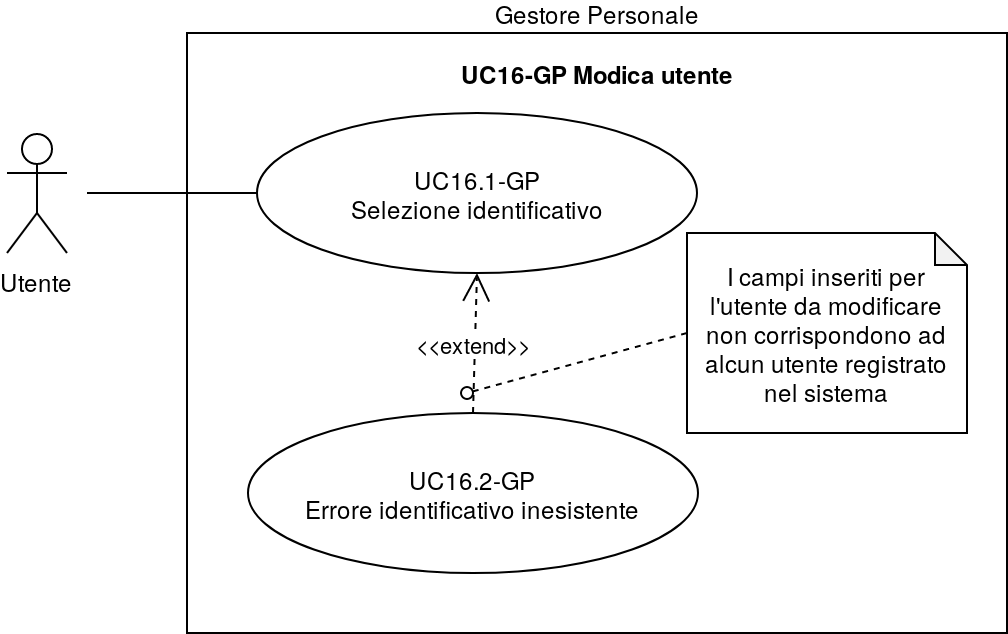
\includegraphics[width=0.8\textwidth]{img/casi_d'uso/UC16.png}\\
			\caption{UC\theuccount-GP - Modifica utente}
		\end{figure}
	\begin{itemize}
		\item \textbf{Codice}: UC\theuccount-GP.
		\item \textbf{Titolo}: modifica utente.
		\item \textbf{Attori primari}: utente.
		\item \textbf{Descrizione}: l’utente vuole modificare le informazioni relative a un altro utente, o di se stesso.
		\item \textbf{Precondizione}: l'utente vuole modificare i dati di un utente già presente nel sistema.
		\item \textbf{Postcondizione}: i campi dell'utente sono stati modificati correttamente.
		\item \textbf{Scenario Principale}:
		\begin{enumerate}
			\item L'utente modifica i dati relativi di un utente
		\end{enumerate}
	\end{itemize}
	
	\stepcounter{subuccount}
	\paragraph{UC\theuccount.\thesubuccount-GP - Selezione identificativo}
		\begin{figure}[H]
			\centering
			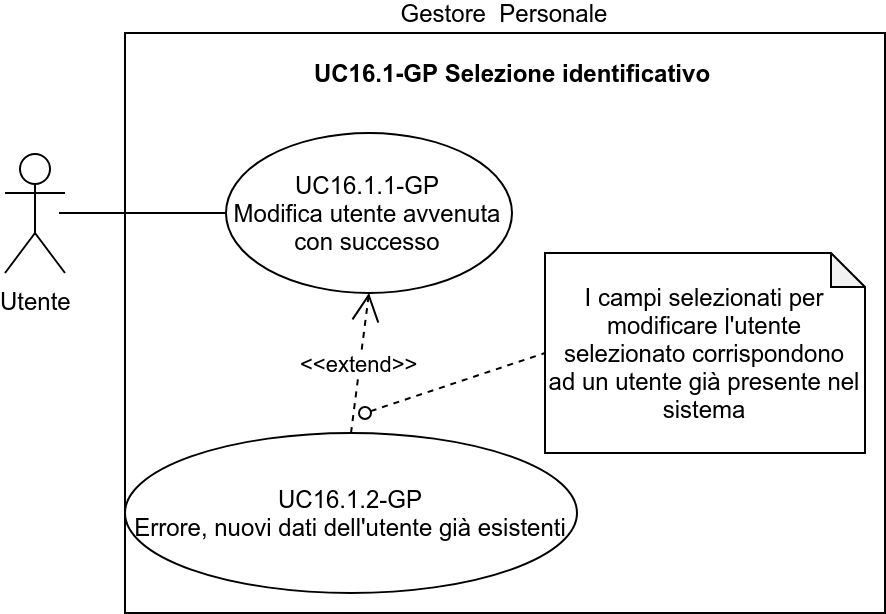
\includegraphics[width=0.8\textwidth]{img/casi_d'uso/UC16_1.png}\\
			\caption{UC\theuccount.\thesubuccount-GP - Selezione identificativo}
		\end{figure}
		\begin{itemize}
			\item \textbf{Codice}: UC\theuccount.\thesubuccount-GP.
			\item \textbf{Titolo}: selezione identificativo.
			\item \textbf{Attori primari}: utente.
			\item \textbf{Descrizione}: l'utente aggiunge l'identificativo dell'utente che vuole modificare.
			\item \textbf{Precondizione}: l'utente vuole modificare un utente già presente.
			\item \textbf{Postcondizione}: l'identificativo è stato inserito.
			\item \textbf{Scenario Principale}:
			\begin{enumerate}
				\item L'utente procede con l'inserimento dell'identificativo dell'utente da modificare
			\end{enumerate}
			\item \textbf{Estensioni}:
			\begin{itemize}
				\item Errore identificativo inesistente [UC\theuccount.2-GP]
			\end{itemize}
		\end{itemize}
		
		\stepcounter{subsubuccount}
		\subparagraph{UC\theuccount.\thesubuccount.\thesubsubuccount-GP - Modifica utente avvenuta con successo}
			\begin{figure}[H]
				\centering
				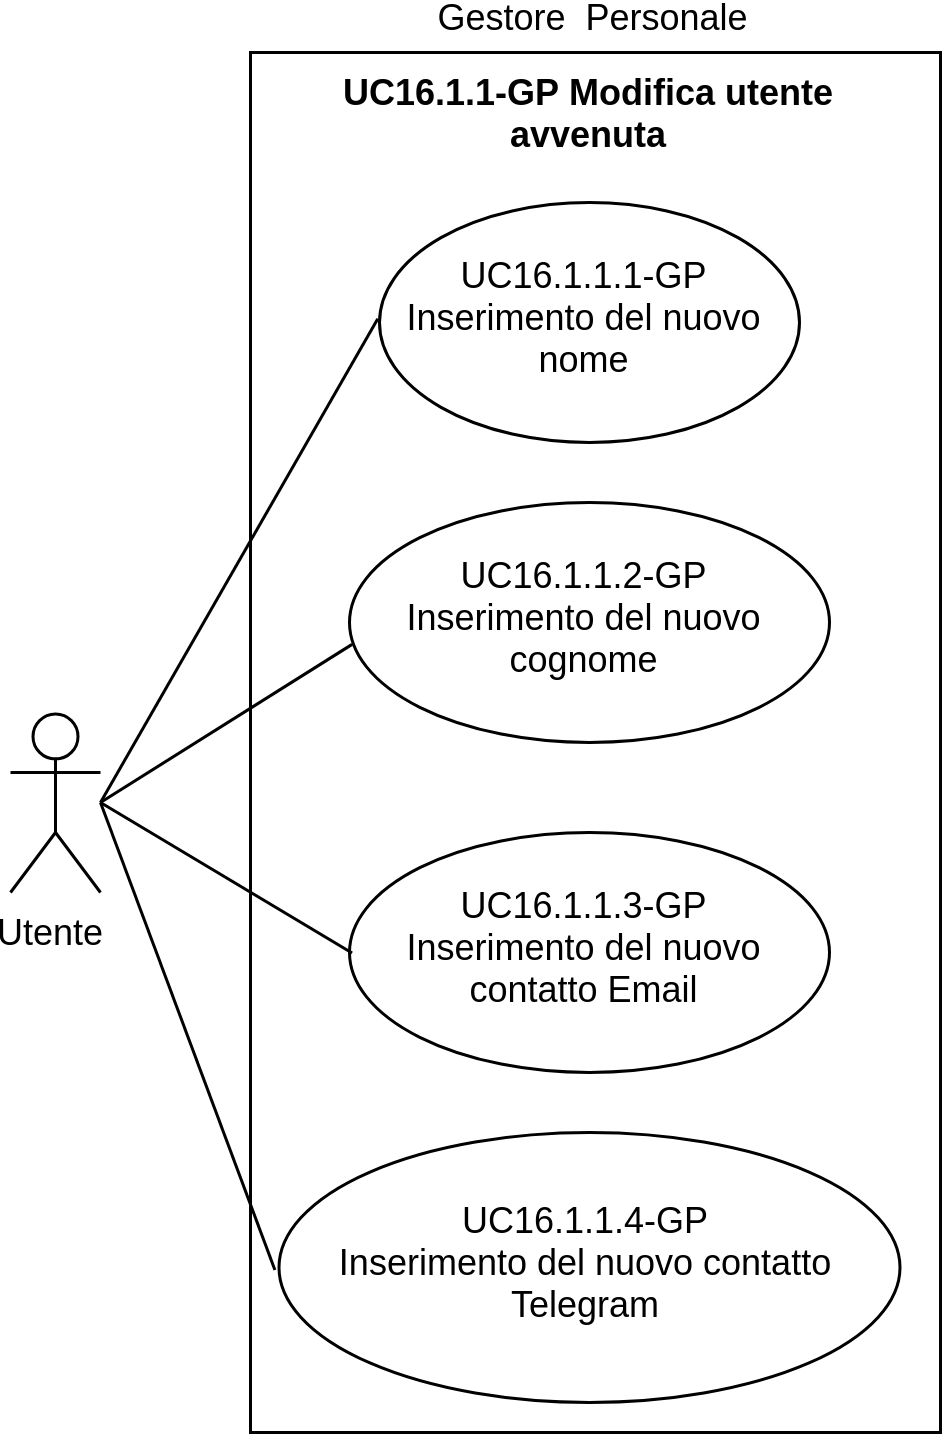
\includegraphics[width=0.5\columnwidth]{img/casi_d'uso/UC16_1_1.png}\\
				\caption{UC\theuccount.\thesubuccount.\thesubsubuccount-GP - Modifica utente avvenuta con successo}
			\end{figure}
			\begin{itemize}
				\item \textbf{Codice}: UC\theuccount.\thesubuccount.\thesubsubuccount-GP.
				\item \textbf{Titolo}: modifica utente avvenuta con successo.
				\item \textbf{Attori primari}: utente.
				\item \textbf{Descrizione}: l'identificativo è presente nel sistema e ne vengono modificati i relativi campi con successo.
				\item \textbf{Precondizione}: l'utente vuole modificare un utente già presente.
				\item \textbf{Postcondizione}: l'utente è stato modificato con successo.
				\item \textbf{Scenario Principale}:
				\begin{enumerate}
					\item L'utente viene modificato con successo
				\end{enumerate}
				\item \textbf{Estensioni}:
				\begin{itemize}
					\item Errore, nuovi dati dell'utente già esistenti [UC\theuccount.\thesubuccount.2-GP]
				\end{itemize}
			\end{itemize}
			
			\stepcounter{subsubsubuccount}
			\subsubparagraph{UC\theuccount.\thesubuccount.\thesubsubuccount.\thesubsubsubuccount-GP - Inserimento del nuovo nome}
				
				\begin{itemize}
					\item \textbf{Codice}: UC\theuccount.\thesubuccount.\thesubsubuccount.\thesubsubsubuccount-GP.
					\item \textbf{Titolo}: inserimento del nuovo nome.
					\item \textbf{Attori primari}: utente.
					\item \textbf{Descrizione}: l'utente aggiunge il nuovo nome relativo all'identificativo inserito che vuole modificare.
					\item \textbf{Precondizione}: l'utente vuole modificare un utente già presente.
					\item \textbf{Postcondizione}: il nome è stato inserito.
					\item \textbf{Scenario Principale}:
					\begin{enumerate}
						\item L'utente inserisce il nuovo nome dell'utente che vuole modificare
					\end{enumerate}
				\end{itemize}
			
			\stepcounter{subsubsubuccount}
			\subsubparagraph{UC\theuccount.\thesubuccount.\thesubsubuccount.\thesubsubsubuccount-GP - Inserimento del nuovo cognome}
				
				\begin{itemize}
					\item \textbf{Codice}: UC\theuccount.\thesubuccount.\thesubsubuccount.\thesubsubsubuccount-GP.
					\item \textbf{Titolo}: inserimento del nuovo cognome.
					\item \textbf{Attori primari}: utente.
					\item \textbf{Descrizione}: l'utente aggiunge il nuovo cognome relativo all'identificativo inserito che vuole modificare.
					\item \textbf{Precondizione}: l'utente vuole modificare un utente già presente.
					\item \textbf{Postcondizione}: il cognome è stato inserito.
					\item \textbf{Scenario Principale}:
					\begin{enumerate}
						\item L'utente inserisce il nuovo cognome dell'utente che vuole modificare.
					\end{enumerate}
				\end{itemize}
			
			\stepcounter{subsubsubuccount}
			\subsubparagraph{UC\theuccount.\thesubuccount.\thesubsubuccount.\thesubsubsubuccount-GP - Inserimento del nuovo contatto Email}
				
				\begin{itemize}
					\item \textbf{Codice}: UC\theuccount.\thesubuccount.\thesubsubuccount.\thesubsubsubuccount-GP.
					\item \textbf{Titolo}: inserimento del nuovo contatto Email.
					\item \textbf{Attori primari}: utente.
					\item \textbf{Descrizione}: l'utente aggiunge il nuovo contatto Email relativo all'identificativo inserito che vuole modificare.
					\item \textbf{Precondizione}: l'utente vuole modificare un utente già presente.
					\item \textbf{Postcondizione}: il contatto Email è stato inserito.
					\item \textbf{Scenario Principale}:
					\begin{enumerate}
						\item L'utente inserisce il nuovo contatto Email dell'utente che vuole modificare
					\end{enumerate}
				\end{itemize}
			
			\stepcounter{subsubsubuccount}
			\subsubparagraph{UC\theuccount.\thesubuccount.\thesubsubuccount.\thesubsubsubuccount-GP - Inserimento del nuovo contatto Telegram}
				
				\begin{itemize}
					\item \textbf{Codice}: UC\theuccount.\thesubuccount.\thesubsubuccount.\thesubsubsubuccount-GP.
					\item \textbf{Titolo}: inserimento del nuovo contatto Telegram.
					\item \textbf{Attori primari}: utente.
					\item \textbf{Descrizione}: l'utente aggiunge il nuovo contatto Telegram relativo all'identificativo inserito che vuole modificare.
					\item \textbf{Precondizione}: l'utente vuole modificare un utente già presente.
					\item \textbf{Postcondizione}: il contatto Telegram è stato inserito.
					\item \textbf{Scenario Principale}:
					\begin{enumerate}
						\item L'utente inserisce il nuovo contatto Telegram dell'utente che vuole modificare
					\end{enumerate}
				\end{itemize}
			
		\stepcounter{subsubuccount}
		\subparagraph{UC\theuccount.\thesubuccount.\thesubsubuccount-GP - Errore, nuovi dati dell'utente già esistenti}
		
		\begin{itemize}
			\item \textbf{Codice}: UC\theuccount.\thesubuccount.\thesubsubuccount-GP.
			\item \textbf{Titolo}: errore, nuovi dati dell'utente già esistenti.
			\item \textbf{Attori primari}: utente.
			\item \textbf{Descrizione}: i nuovi dati dell'utente da modificare che sono stati inseriti sono già presenti nel sistema.
			\item \textbf{Precondizione}: l'utente vuole modificare un utente già presente.
			\item \textbf{Postcondizione}: l'utente non è stato modificato.
			\item \textbf{Scenario Principale}:
			\begin{enumerate}
				\item L'utente non viene modificato perché i nuovi campi corrispondono a quelli di un utente già esistente
			\end{enumerate}
		\end{itemize}
	\stepcounter{subuccount}
	\paragraph{UC\theuccount.\thesubuccount-GP - Errore identificativo inesistente}
		
		\begin{itemize}
			\item \textbf{Codice}: UC\theuccount.\thesubuccount-GP.
			\item \textbf{Titolo}: errore identificativo inesistente.
			\item \textbf{Attori primari}: utente.
			\item \textbf{Descrizione}:  l’utente viene avvisato che ha inserito un'identificativo errato.
			\item \textbf{Precondizione}: l'utente vuole modificare un utente già presente.
			\item \textbf{Postcondizione}: il sistema comunica all’utilizzatore l’errore.
			\item \textbf{Scenario Principale}:
			\begin{enumerate}
				\item L'utente ha inserito un identificativo errato e il sistema comunica all’utilizzatore l’errore.
			\end{enumerate}
		\end{itemize}